\chapter{Analiza nawiązanej komunikacji}
    \begin{figure}[h!]
        \centering
        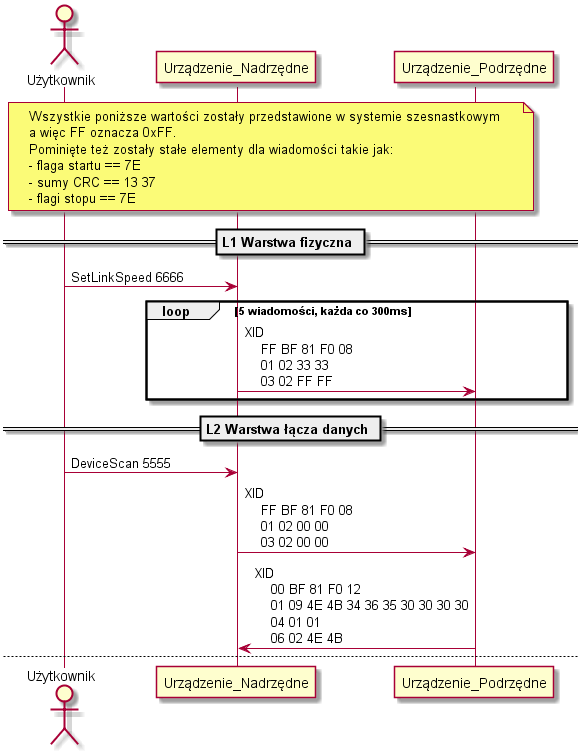
\includegraphics[scale=0.70]{out/Diagramy/UML_DiagramOfSequence_New/UML_DiagramOfSequence_New-page1.png}
        \caption{Ustanowienie prędkości połączenia wraz z początkowym skanowaniem urządzeń
            \newline(Opracowanie własne)}
        \label{fig:DiagramSequence_LinkSpeed_DeviceScan}
        \end{figure}
    \newpage
    W celu szczegółowej analizy wykonania programu przedstawionego na listingu \ref{lst:WykonanieProgramu}, utworzono diagram sekwencji podzielony na kilka części 
    (rysunek \ref{fig:DiagramSequence_LinkSpeed_DeviceScan}),
    co pozwoliło zobrazować zaistniałą komunikację pomiędzy użytkownikiem, urządzeniem nadrzędnym oraz urządzeniem podrzędnym.
    Na diagramie oraz podczas analizy pominięto cztery bajty stałe dla każdej wiadomości, czyli bajt startu równy 0x7E, dwa bajty sumy CRC =\{ 0x13, 0x37\} ( powód dlaczego ta wartość jest stała przedstawiono
    w podsumowaniu ) oraz bajt stopu równy 0x7E.
    \section{Ustanowienie prędkości połączenia}
    Parametrem tej komendy jest adres portu 6666, z którego korzysta sterownik do nawiązania połączenia typu tcp na adresie 127.0.0.1 wraz z symulatorem urządzenia
    przy zastosowaniu wzorca Publikuj-Subskrybuj. Podczas tego połączenia protokół AISG 2.0 nie zakłada oczekiwania na odpowiedź od urządzenia podrzędnego oraz użyta biblioteka
    ZeroMQ również nie udostępnia możliwości wysłania odpowiedzi na taką wiadomość.
    \newline
	Analiza wartości wiadomości wychodzącej (rysunek \ref{lst:WykonanieProgramu}- linijki [3; 12]):
	\begin{enumerate}
        \item ADDR = 0xFF --- \textit{broadcast};
        \item CTRL = 0xBF --- charakterystyczny dla ramki XID;
        \item FI = 0x81 --- charakterystyczna dla ramki XID oraz grupy wiadomości przypisania adresu;
        \item GI = 0xF0 --- grupa wiadomości przypisania adresu;
        \item GL = 0x08;
    \end{enumerate}
    Pominięto analizę kolejnych bajtów dla tej wiadomości % TODO
